\begin{figure}
    \centering
    \begin{subfigure}[b]{0.475\textwidth}
        \centering
        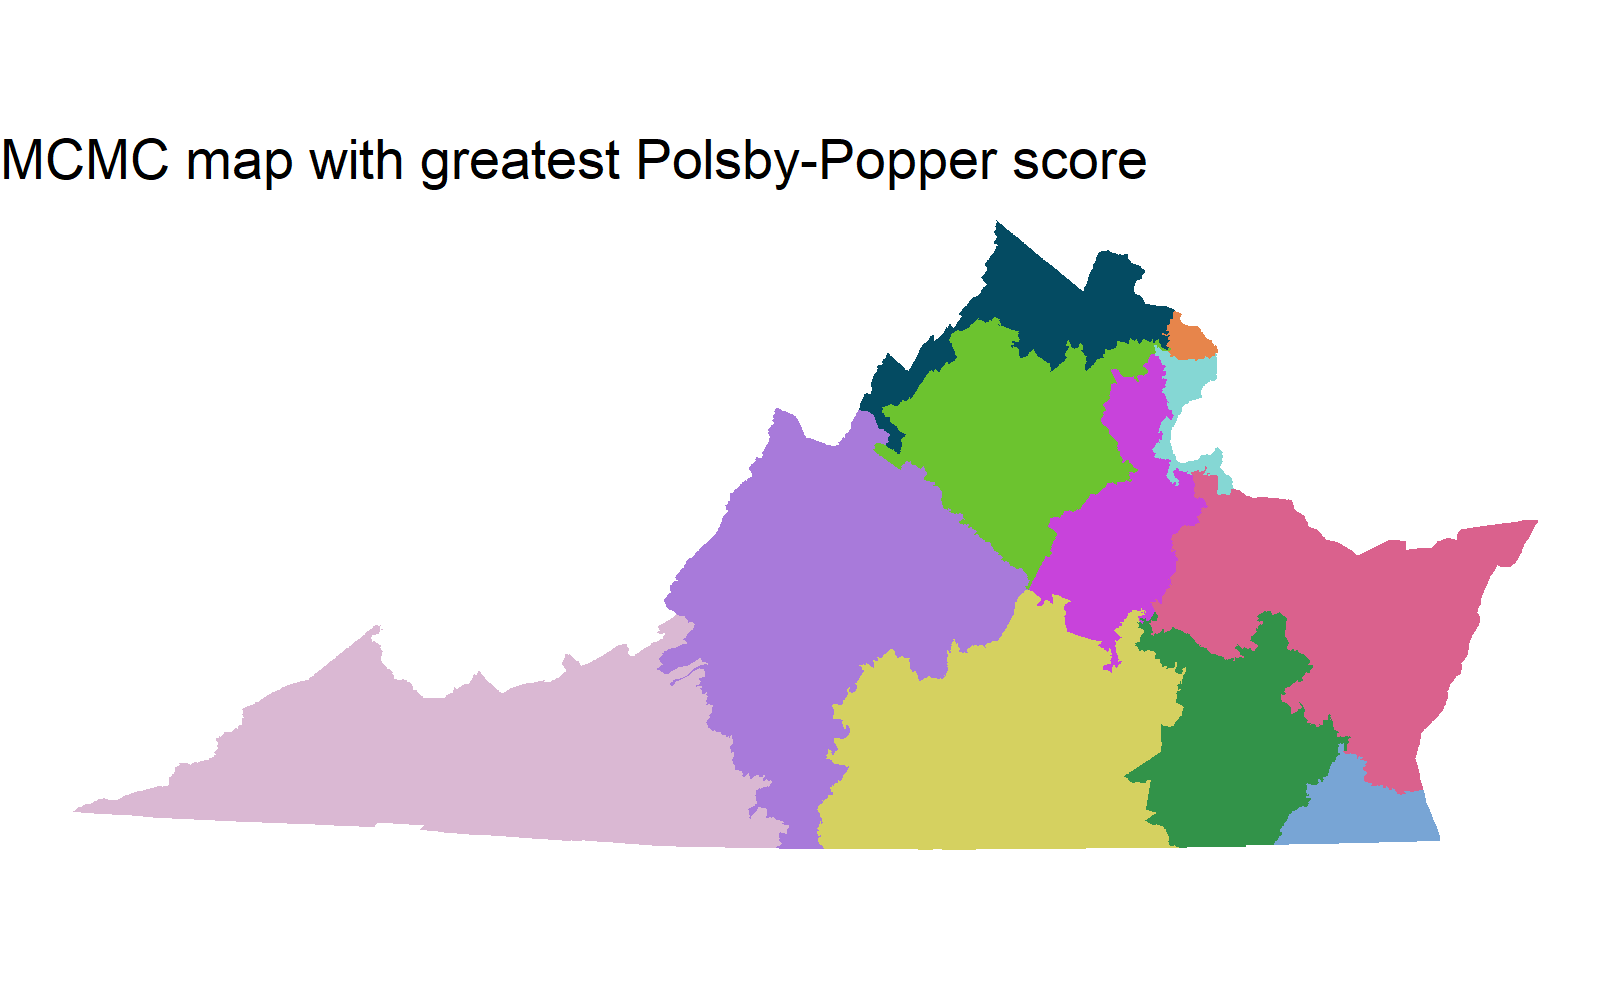
\includegraphics[width=\textwidth]{img/map.mcmc.pp.png}
        \caption{MCMC Map with Greatest Polsby-Popper Score}
        \label{fig:map.mcmc.pp}
    \end{subfigure}
    \hfill
    \begin{subfigure}[b]{0.475\textwidth}
        \centering
        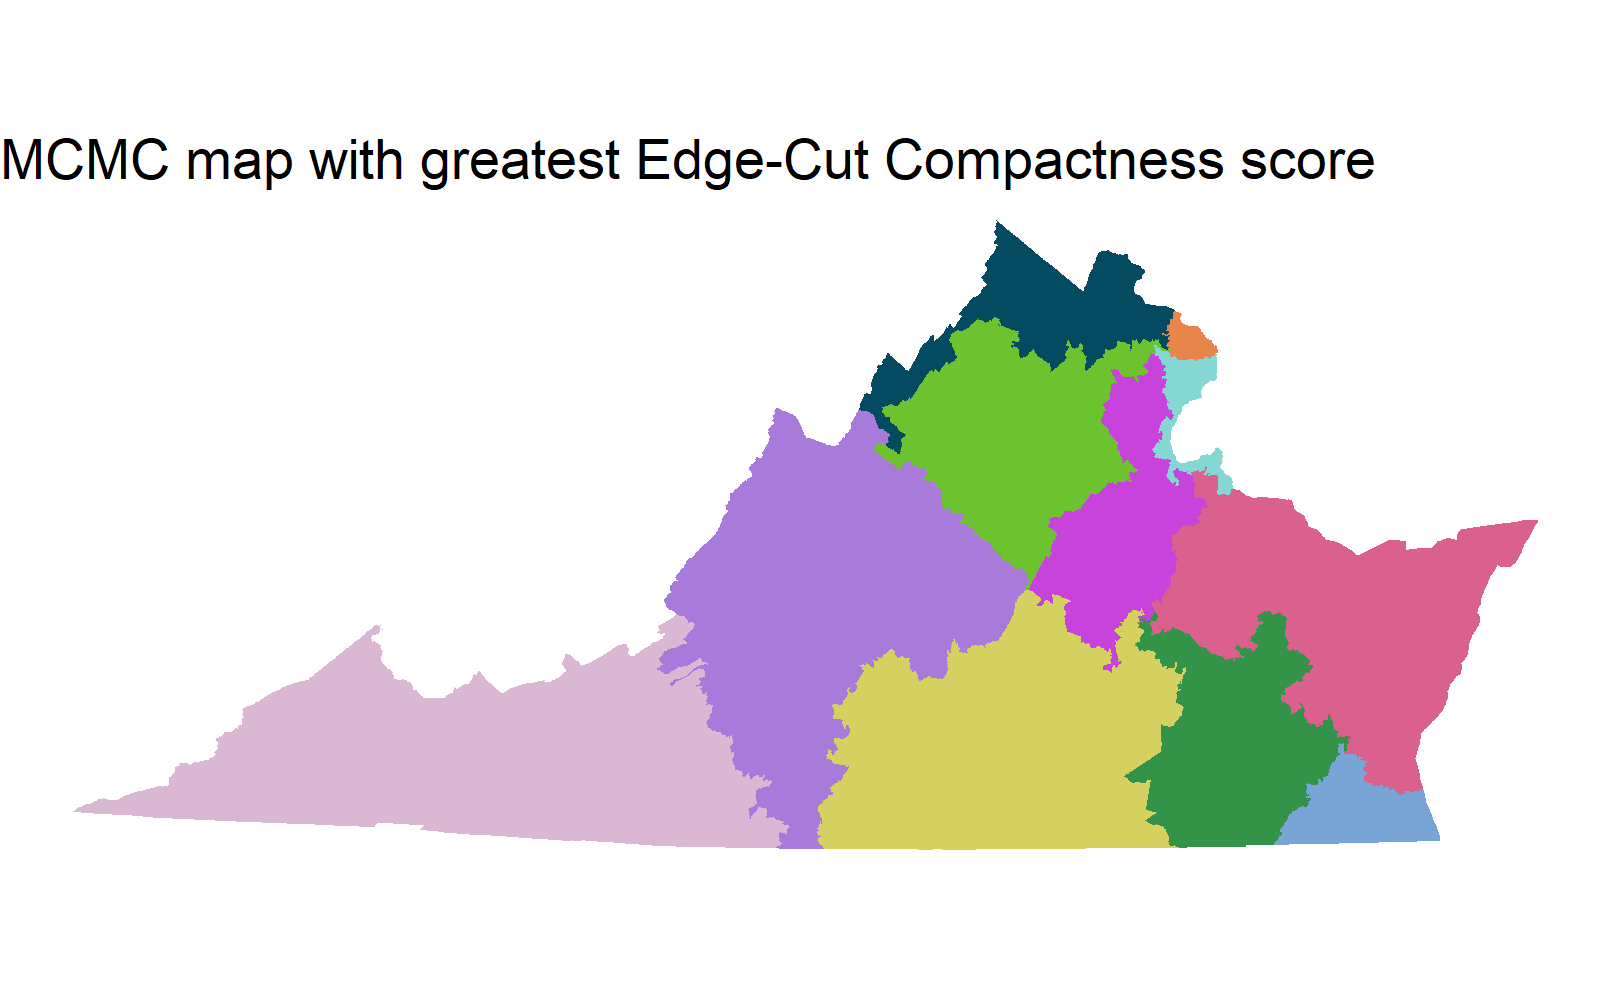
\includegraphics[width=\textwidth]{img/map.mcmc.ecc.png}
        \caption{MCMC Map with Greatest Edge-Cut Compactness Score}
        \label{fig:map.mcmc.ec}
    \end{subfigure}
    \vskip\baselineskip
    \begin{subfigure}[b]{0.475\textwidth}
        \centering
        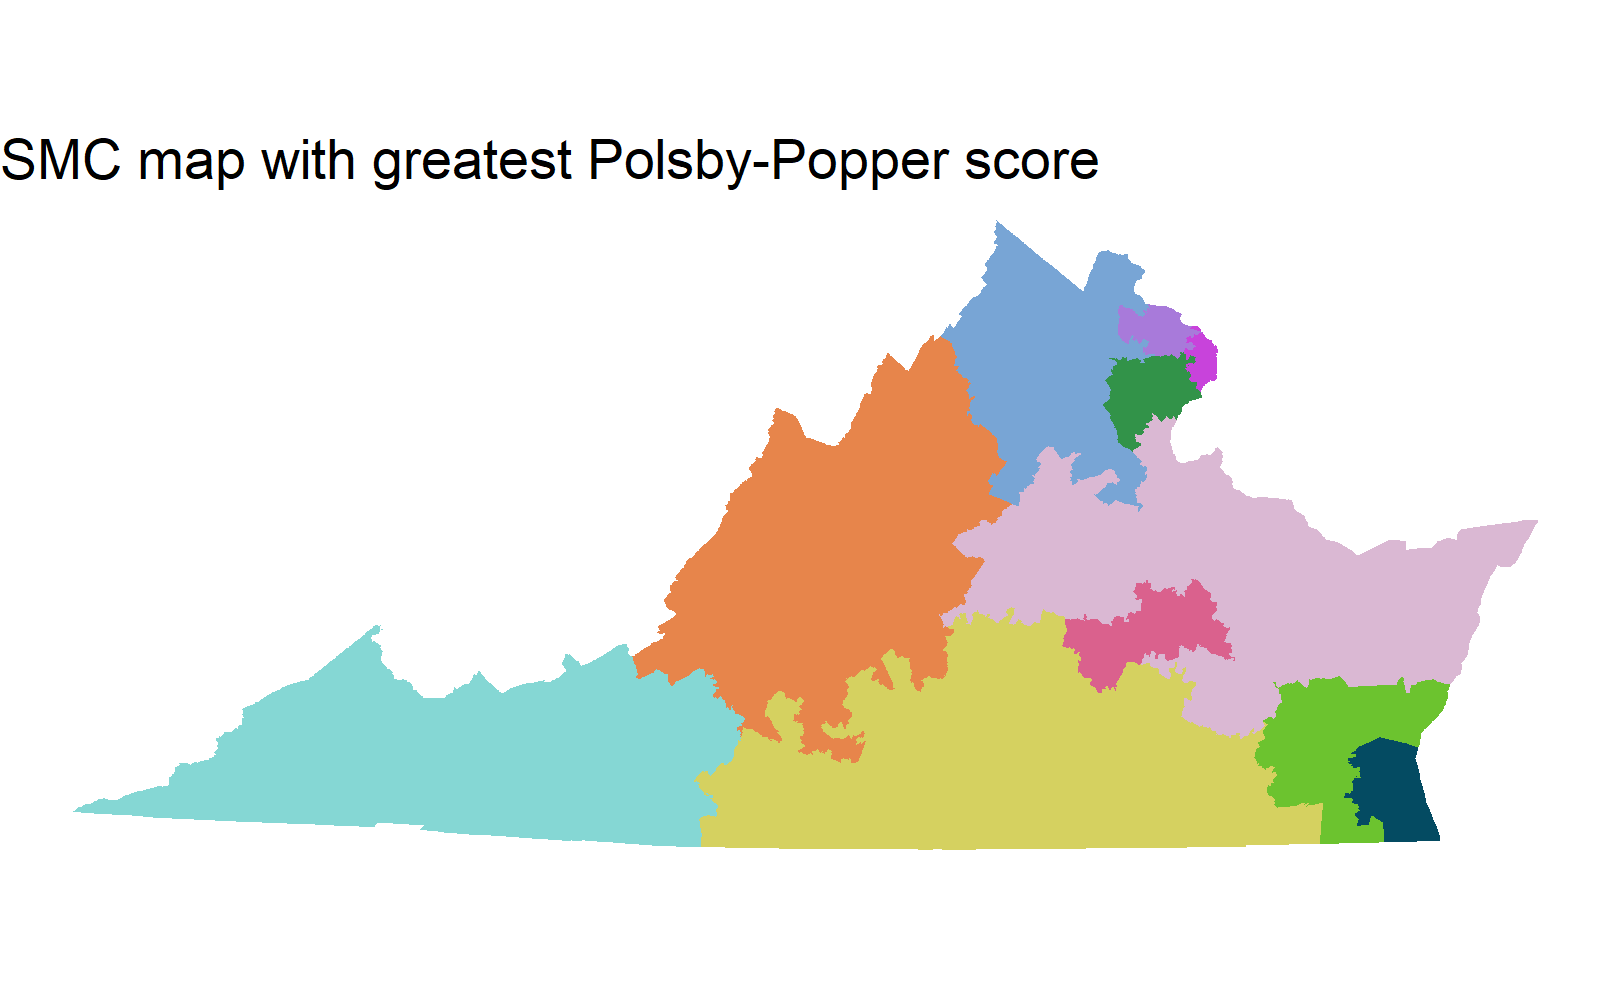
\includegraphics[width=\textwidth]{img/map.smc.pp.png}
        \caption{SMC Map with Greatest Polsby-Popper Score}
        \label{fig:map.smc.pp}
    \end{subfigure}
    \hfill
    \begin{subfigure}[b]{0.475\textwidth}
        \centering
        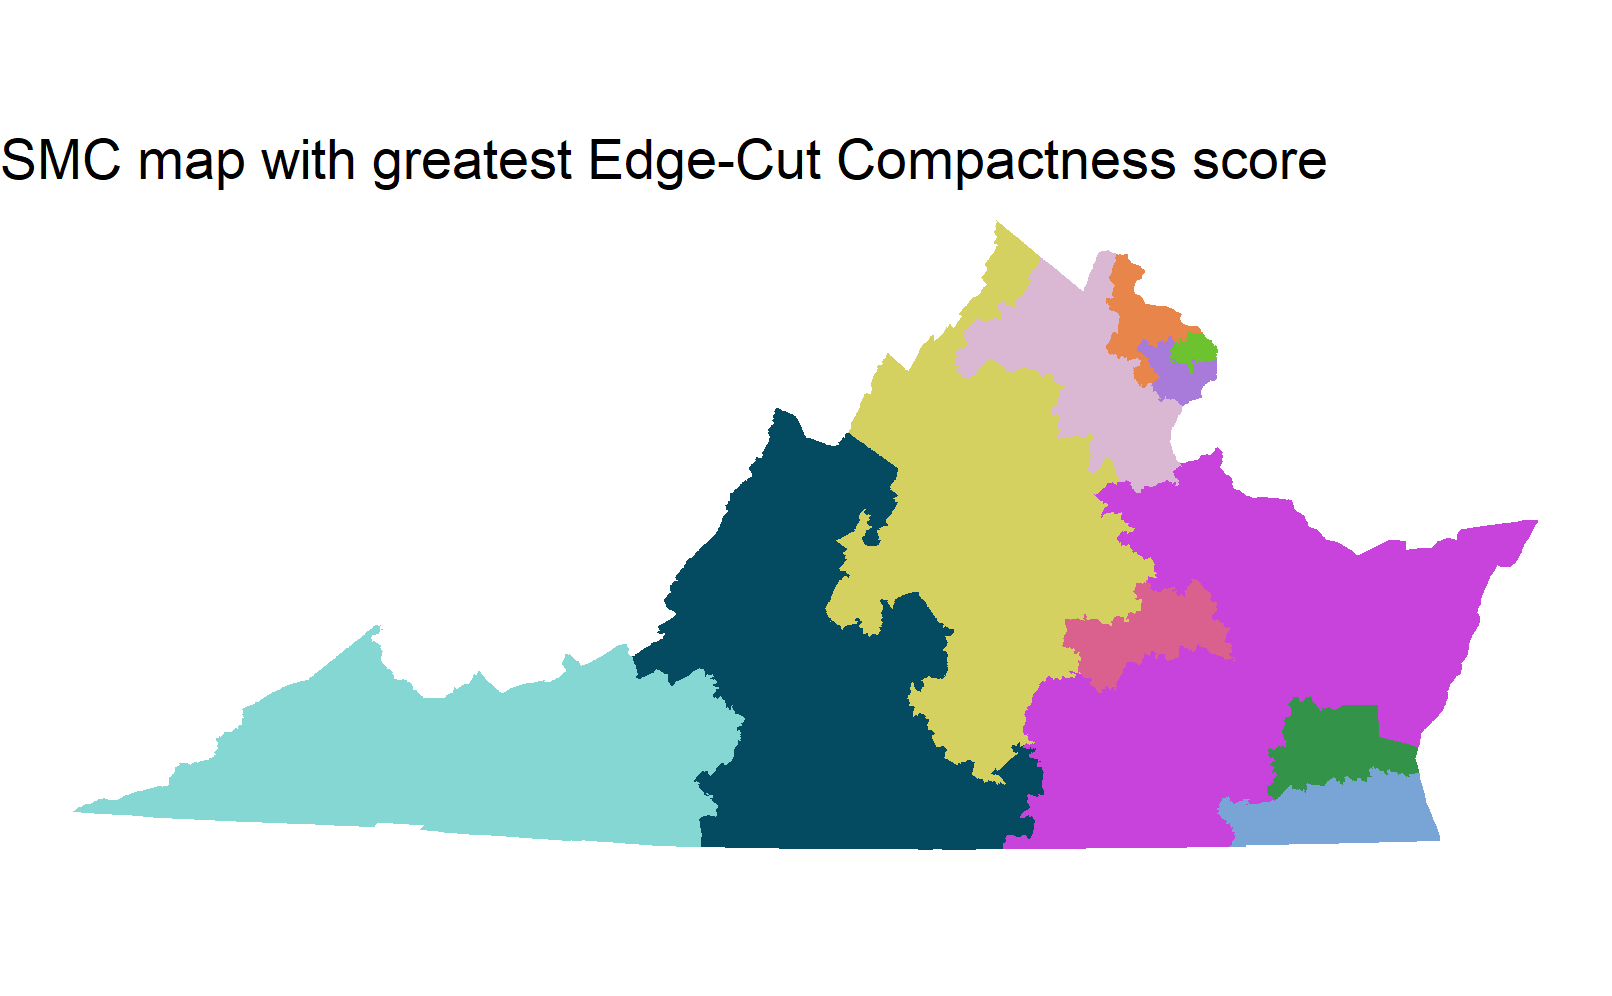
\includegraphics[width=\textwidth]{img/map.smc.ec.png}
        \caption{SMC Map with Greatest Edge-Cut Compactness Score}
        \label{fig:map.smc.ec}
    \end{subfigure}
    \vskip\baselineskip
    \begin{subfigure}[b]{0.475\textwidth}
        \centering
        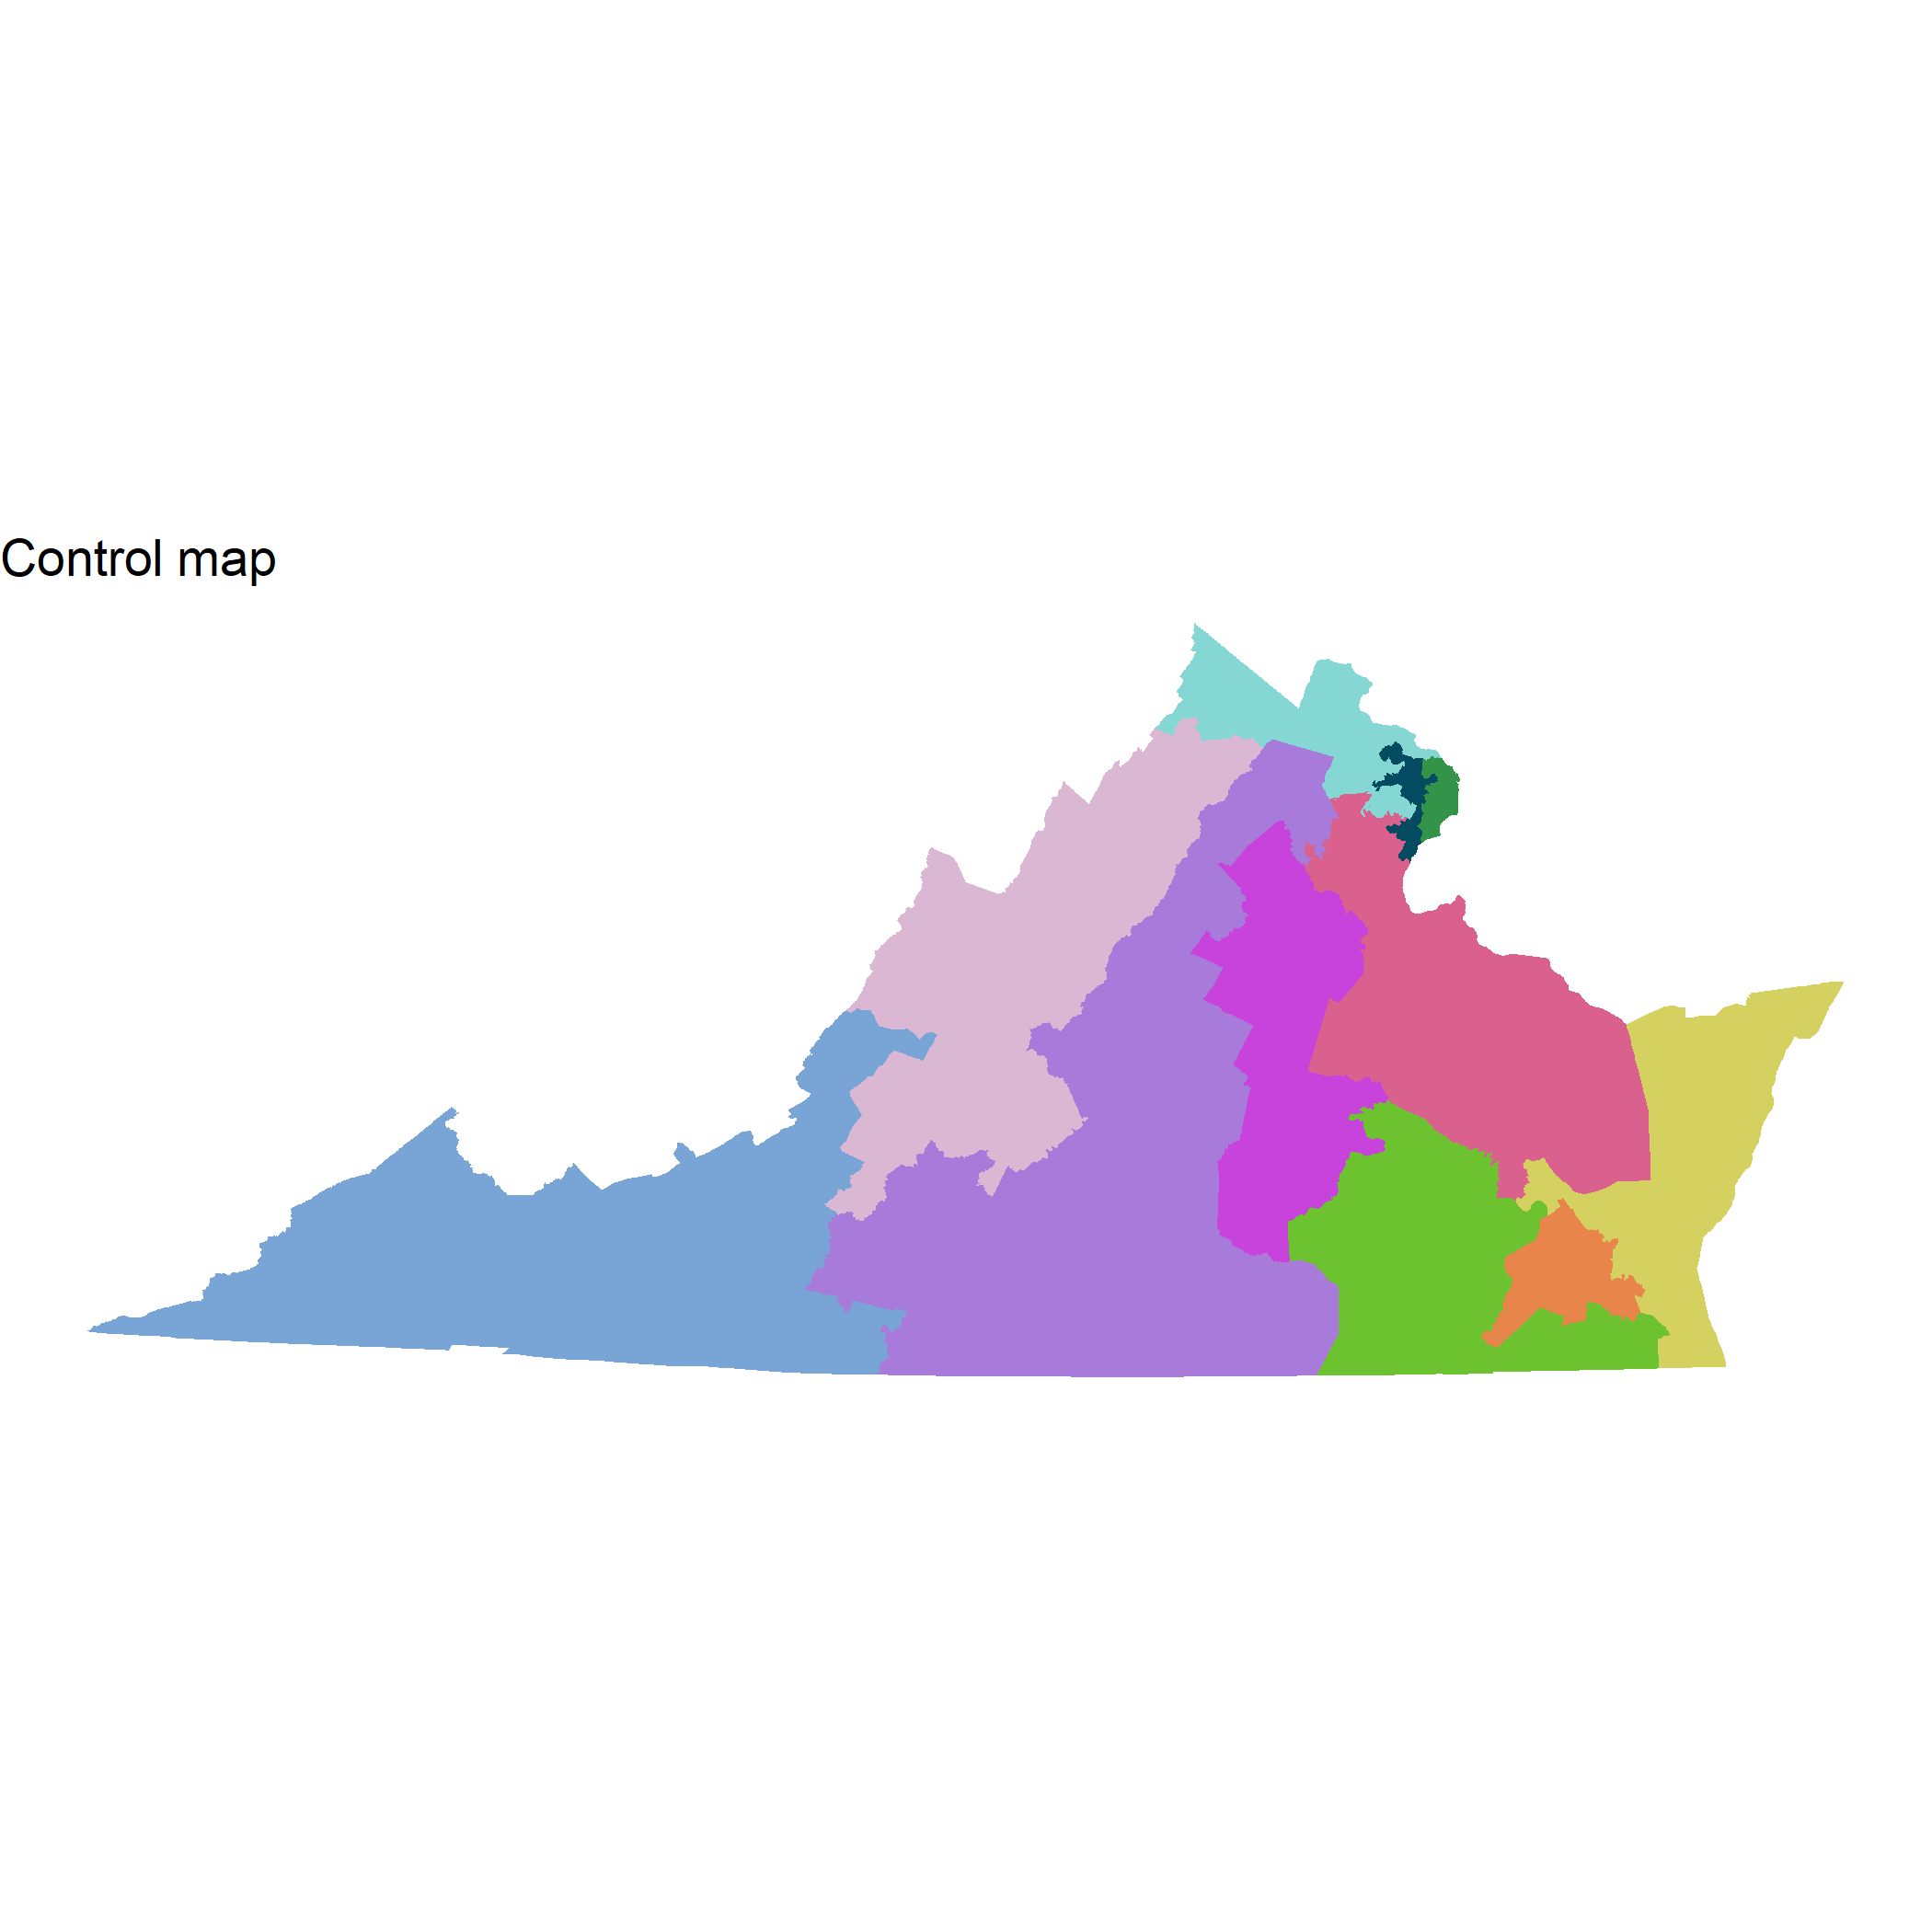
\includegraphics[width=\textwidth]{img/map.control.png}
        \caption{Control Map}
        \label{fig:map.control}
    \end{subfigure}
       \caption{Maps of Most Compact Redistricting Plans}
       \label{fig:maps}
\end{figure}